\chapter{Тестирование и апробация плагина в Jenkins} \label{ch4}

% не рекомендуется использовать отдельную section <<введение>> после лета 2020 года
%\section{Введение. Сложносоставное название первого параграфа первой главы для~демонстрации переноса слов в содержании} \label{ch1:intro}

В главе описано проведенное тестирование и апробация плагина:

\begin{enumerate}
	\item Описаны методы тестирования.
	
	\item Проведена апробация плагина в системе Jenkins.
	
	\item Разработан код тестирования плагина.
	
	
	
\end{enumerate}

\section{Методы тестирования} \label{ch4:sec1}

Тестирование программного обеспечения — обширное понятие, которое включает планирование, проектирование и, собственно, выполнение тестов  \cite{testing}. В процессе CI/CD производится непрерывное тестирование разработанного кода, а также тестирование разработанного приложения. Сам плагин является частью CI/CD процессе, но также требует тестирования корректной работы своей функциональности, тестирование разработанного кода, а также тестирования на соответствие исходным требования, которые были предъявлены к разработке в главе 1.

Существует множество методов тестирования и техник тест дизайна, в процессе анализ функциональных требования были отобраны те, которые наиболее релевантные для разработанного плагина Jenkins.

Будет проведено как ручное, так и автоматизированное тестирование плагина. Ручное тестирование поможет выявить нетипичные тест-кейсы, которые не покрываются автоматизированными тестами.

Ручные тесты будут проведены методом черного ящика. Данный метод это процедура получения и выбора тестовых случаев на основе анализа функциональности и технического задания, без применения знаний о внутреннем устройстве системы \cite{blacktest}.

Были составлены тест-кейсы, которые отражены в таблице 4.1.

\begin{table}
    \centering
    \caption{Составленные тест-кейсы}
    \begin{tabular}{|p{1cm}|p{5cm}|p{9cm}|}
    \hline
        № & Описание & Ожидание  \\ \hline
        1 & Проверка выбранного периода на графике SR (месяц) & Количество  дней соответствует прошлому месяцу, на каждый день отображены корректные значения процента успешности сборок\\ \hline
        2 & Проверка выбранного периода на графике BD (неделя) с учетом выбора настройки среднего значения и  упавших сборок& Количество  дней 7 в соответствии со всеми днями недели, на каждый день отображены корректные значения среднего времени продолжительности сборок, учтены упавшие сборки \\ \hline
        3 & Проверка выбранного периода на графике TQ (квартал) с учетом выбора настройки среднего значения & Количество  кварталов 4 в соответствии с кварталами года, на каждый квартал отображены средние значения проведенного в очереди времени сборок  \\ \hline
        4 & Проверка выбранного периода на графике TC (год) с учетом выбора настройки упавших сборок & Количество  месяцев 12 соответствует прошедшему году, на каждый месяц отображены корректные значения  количества тестов, с учетом тестов выполненных на упавших сборках \\ \hline
        5 & Проверка выбранного периода на графике AS (день) & Количество  часов 24 соответствует всем часам прошедшего дня, на каждый час отображены корректные значения размера итоговых артефактов полученного по результатам задания   \\ \hline
        6 & Проверка корректного отображения при выборе периода ALL & Отображены сборки со всего периода прошедшего, информация поделена на равное части   \\ \hline
        7 & Проверка корректного отображения аномальных значений & Отображены номера сборок, возле каждого графика, у которых аномальное значений метрики соответствующей графику   \\ \hline
        8 & Проверка корректного расчета предугаданной 'следующей' сборки& Метрики предугаданной сборки рассчитываются корректно для каждого графика   \\ \hline

    \end{tabular}
\end{table}

В данном случае тест-кейсы были описаны с помощью техники тест-дизайна Матрица трассировки. Если обратиться к определению, то матрица трассировки — двумерная таблица, содержащая соответствие функциональных требований и подготовленных тестовых сценариев \cite{matrixtest}, а на пересечении столбцов и строк ставится метка, о том, что данное требование покрывается данным тест-кейсом. В случае данной работы из соображений удобства и оптимизации тестовой документации, было принято решение модифицировать матрицу трассировки и совместить с подробным описание в формате чек листа: для оптимизации идет проверка, что каждый тип графика-метрики (Success Rate) корректно себя ведет на определенном периоде (неделя), таким образом не придется проверять, каждый график на каждом периоде при каждой доработке кода продукта.

Данные тест-кейсы оптимизированы, поскольку в соответствии с пирамидой тестирования \cite{TestPyramid} ручные UI кейсы, находятся в самой верхней ее части и не должны занимать достаточно большое место в системе тестирования. С дрогой стороны для улучшения покрытия требования, предъявляемых к продукты должны использоваться гораздо в большем объеме unit-тесты, т.е. тесты в которых самые маленькие компоненты системы - модули (модули, классы, методы), индивидуально проверяются на предмет правильной работы \cite{unittest}.

\subsection{Unit тестирование}

При написание юнит тестов используется метод белого ящика. Данный метод предоставляет тестировщику полное знание тестируемого приложения, включая доступ к исходному коду и проектной документации \cite {whitebox}, т.е. тестирование происходит на основе знания исходного кода, таким образом, юнит тестирование методом белого ящика поможет нам достаточно широко покрыть все модули плагина. Для запуска тестов требуется перейти в корень директории плагина и выполнить команду mvn test.

Код юнит тестов расположен в классе BuildConfigurationStatisticsBuilderTest. В этом классе проводятся проверки, такие как:

\begin{itemize}
	\item проверка корректности системы в целом - testWorkingSystem();
	\item проверка успешного завершения сборки - testSuccessBuildFromCustomBuild();
	\item проверка падения сборки при некорректных входных данных - testFailBuildFromCustomBuild();
	\item проверка формирования структур для начальной инициализации данных - testCreateDateWeekMapSuccessRate(), testCreateDateMonthMap();
	\item проверки корректности написанных методов работы с датой - testDateMonthToString(), testGetLastMonthDays();
	\item проверка работоспособности модулей обработки времени сборок - testGetTimeInQueue().
\end{itemize}

Код юнит тестов приведен в приложении 5.

\subsection{UI тестирование}

Также для автоматизации тестирования UI части плагина, был применен Selenium web driver и язык программирования python. WebDriver управляет браузером, как это делает пользователь, с использованием сервера Selenium \cite{webdriver}. Данные тест-кейсы будут в автоматическом режиме проверять реакцию элементов веб интерфейса на действия пользователя. Для запуска тестов требуется перейти в корень проекта Selenium и запустить команду pytest, при необходимости указать браузер и url, с которыми необходимо запустить UI тесты.

Код UI тестов расположен в отдельном проекте в классе TestCase. В этом классе проводятся проверки, такие как:

\begin{itemize}
	\item проверка корректности открытия и наличия элементов во вкладке на странице плагина - test\_open\_tab(self);
	\item проверка наличия и корректного отображения графика SR - test\_success\_rate\_chart(self);
	\item проверка наличия и корректного отображения графика BD - test\_build\_duration\_chart(self);
	\item проверка наличия и корректного отображения графика TC - test\_test\_count\_chart(self);
	\item проверка наличия и корректного отображения графика BQ - test\_time\_spent\_queue\_chart(self);
	\item проверка наличия и корректного отображения графика AS - test\_artifacts\_size\_chart(self);
	\item проверка корректности реакция элемента выпадающего списка - test\_change\_value\_select\_period(self);
	\item проверка  корректности реакция чекбоксов - test\_change\_value\_checkbox(self).
\end{itemize}

Код UI тестов приведен в приложении 6.



 \section{Апробация плагина} \label{ch4:sec2}
 
 Апробация плагина будет проводится в системе CI Jenkins для которой и был разработан плагин визуализации. Для того чтобы провести апробацию плагина на локальном сервере Jenkins, запущенном на локальном или удаленном ПК, потребуется произвести несколько операций. Для начала, нужно будет клонировать репозиторий с кодом плагина на GitHub, перейти в папку проекта и выполнить \cite{deployplugin} Maven mvn install и скопировать .hpi в папку /plugins/. 
 
 Затем потребуется на запущенном сервере Jenkins перейти в Управление Jenkins  и среди доступных плагинов выбрать Build Configuration Statistics, установить, после чего напротив каждой сборки Jenkins в боком меню, откуда можно запустить и отредактировать сборку, появится пункт меню Build Configuration Statistics, при нажатии на которой должны отобразиться все графики с собранной статистикой по метрикам каждого задания в Jenkins. 
 
 \subsection{Подготовка и генерация набора сборок для апробации}
 
 Для того чтобы графики отображали какие-то данные, необходимо сначала сгенерировать сборки разной длительности, статусов, с разным количеством тестов и размером артефактов.
 
Для генерации запусков сборки, можно задать конфигурацию сборки через меню Configuration, а затем с помощью действия Build Now в меню сборки, запустить сборку на выполнение. Также можно использовать плагин Pipeline, для того чтобы декларативно с помощью groovy скрипта задать конфигурацию сборки с шагами, которые будут выполнять при запуске сборки. 

Пример скрипта для создания для создания сборки, в которой будет выполняться два шага: создание файла и создания артефакта сборки из созданного файла с помощью cmd Windows.

\begin{lstlisting}
pipeline {
    agent any
    stages {
        stage('Create file') {
            steps {
                bat 'echo Hello World > myfile.txt'
            }
        }
        stage('Archive file') {
            steps {
                archiveArtifacts artifacts: 'myfile.txt', onlyIfSuccessful: true
            }
        }
    }
}
\end{lstlisting}

Для того чтобы проверить корректность обработки данных во времени, можно после запуска сборки, отредактировать (в логах выбранного запуска в папке запуска в файле build.xml) xml теги   <timestamp>1684077728000</timestamp> и
  <startTime>1684077728013</startTime> , в которых в формате timestamp задать нужное время в прошлом. Для конвертации даты и времени в timestamp можно использовать веб-ресурс https://www.epochconverter.com/.
  
Например, для даты Sunday, May 14, 2023 3:22:08 PM получаем следующий результат в формате timestamp 1684077728000 в миллисекундах. После редактирования xml файла с информацией о сборке получим необходимое дату  и время в интерфейсе Jenkins. Пример отредактированной сборки с датой в прошлом указан на рисунке 4.1.

 \begin{figure}[ht!] 
	\center
	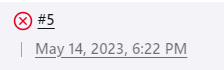
\includegraphics [scale=0.87] {my_folder/images//lastBuild}
	\caption{Сборка с датой в прошлом} 
	\label{fig:lastBuild}  
\end{figure}
 
 В ходе апробации плагина были сгенерированы сборки, которые отображены на рисунке 4.2.
 
 \begin{figure}[ht!] 
	\center
	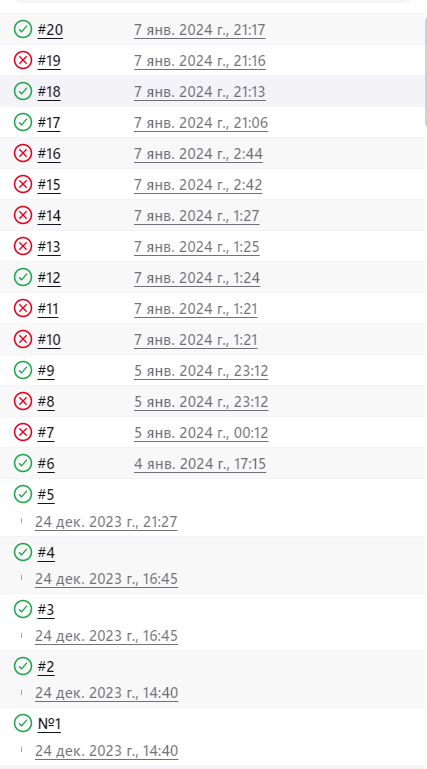
\includegraphics [scale=0.47] {my_folder/images//builds}
	\caption{Сгенерированные сборки} 
	\label{fig:builds}  
\end{figure}

Запуски были сгенерированы с разной датой начала:

\begin{itemize}
	\item 5 успешных запусков с датой 24.12.2023, с разным временем начала с 2 до 9 часов вечера;
	\item 1 успешный запуск 4.01.2024;
	\item 3 запуска 5.01.2024 - 2 из которых закончилось с результатом падение (в 0 часов и 23 часа), а один с положительным результатом в 23 часа;
	\item 11 запусков 7.01.2024 из которых 7 закончилось падением, а 4 с успешным результатом, запуски имеют разное время начала с 1 до 21 часа ;
	\item 2 запуска 11.01.2024 один из которых закончился падением с временем начала 14 часов, а другой с успешным результатом в 14 часов;
	\item 2 успешных запуска 12.01.2024 со временем начала 13 часов и 16 часов.
\end{itemize}


 Среди сборок присутствуют, упавшие сборки со специально завышенным временем выполнения 100 секунд, сборки без завышенного времени выполнялись около 20 секунд. Такая сборка отображена на рисунке 4.3.
 
 \begin{figure}[ht!] 
	\center
	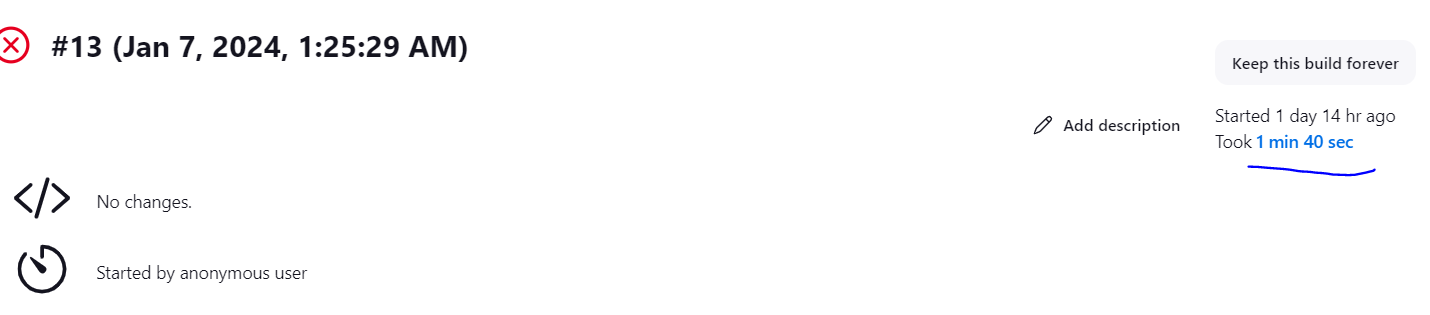
\includegraphics [scale=0.47] {my_folder/images//longBuild}
	\caption{Длинная упавшая сборка} 
	\label{fig:longBuild}  
\end{figure}


А также сборки, с созданными артефактами, часть из которых в статусе успешного выполнения, с короткой продолжительностью, а часть из которых завершены падением с большой продолжительностью выполнения. Были определены разные файлы-артефакты для генерации с размером от 70 байт до 1 Кб. Перенос созданных файлов в артефакты выполнялся с помощью конфигурационного разделы в сборке Post-build Actions, в котором выплавлялась команда Archive the artifacts. Сборка с артефактом отображена на рисунке 4.4.
 
 \begin{figure}[ht!] 
	\center
	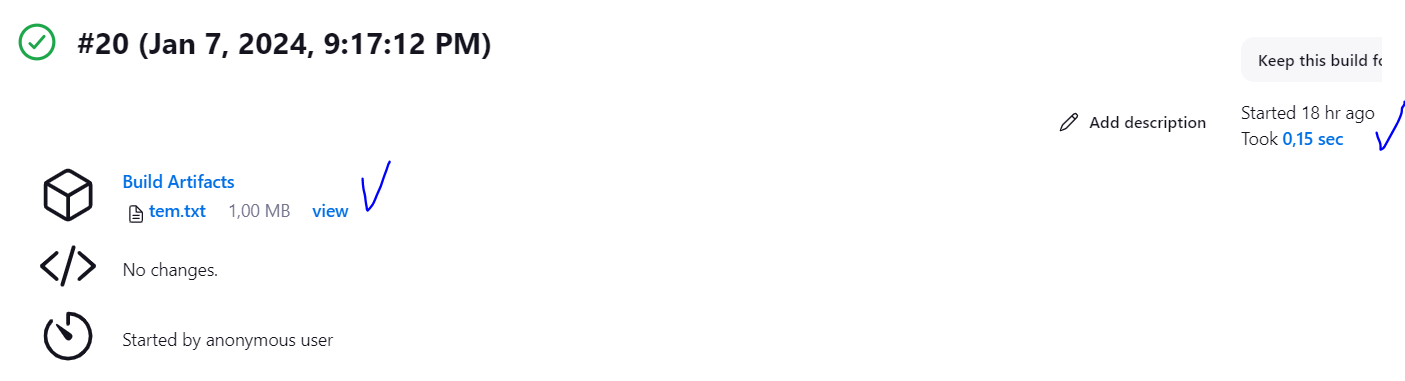
\includegraphics [scale=0.47] {my_folder/images//artifactBuild}
	\caption{Короткая успешная сборка с артефактом} 
	\label{fig:artifactBuild}  
\end{figure}



Часть сборок выполнялось посредством созданного класса в плагине BuildConfigurationStatisticsBuilder, который добавлял еще один вариант запуска шагов сборки Build Steps. Этот класс выполнял вывод информации о текущес запуске в консоль, а также вывод информации с именами всех запусков, уже выполненных в сборке, а также вывод параметра, который задавался при создании шага в конфигурации сборки. Информация из консоли с процессом выполнения шага представлена на рисунке 4.5.

 \begin{figure}[ht!] 
	\center
	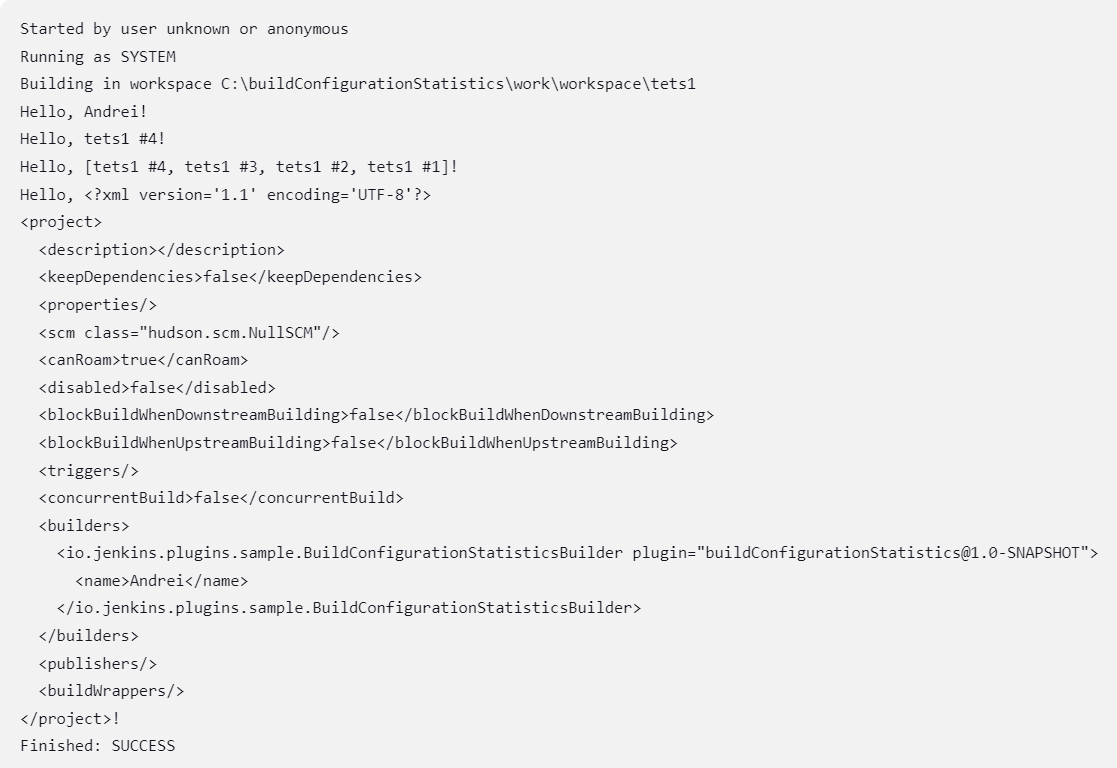
\includegraphics [scale=0.57] {my_folder/images//console1}
	\caption{Консоль шага с разработанным Builder} 
	\label{fig:customBuilder}  
\end{figure}



Для части сборок был добавлен 1 шаг с выполнением cmd команды  \textit{echo 123}, для создания упавших сборок, команды cmd намеренно прописывались с ошибками в синтаксисе, например  \textit{echo1 123}.

Для того чтобы увеличить время выполнения сборок использовалась команда cmd  \textit{waitfor SomethingThatIsNeverHappening /t 100  2>NUL}, которая обеспечивала время выполнения запуска 100 секунд.

Для создания небольших файлов-артефактов использовалась команда cmd \textit{echo "tempbuild1111111111111111111"  1>tembuild.txt}. А для генерация файлов в 1Кб команда \textit{fsutil file createnew tem.txt 1048576}.

\subsection{Апробация на проекте с открытым исходным кодом}

Для того, чтобы убедиться, что плагин работает также на уже существующих проектах, необходимо провести апробацию на стороннем проекте. В качестве такого проекта был выбран frontend-maven-plugin (https://github.com/eirslett/frontend-maven-plugin). 

Это плагин, который загружает/устанавливает Node и NPM локально для вашего проекта, запускает npm install, а затем любую комбинацию Bower , Grunt , Gulp , Jspm , Karma или Webpack и может работать в Windows, OS X и Linux \cite{frontplugin}. У проекта 865 forks на GitHub, а также более 4 тысяч звезд, из чего следует, что его разработка была полезна для ИТ сообщества и активно используется разработчиками.

Следуя, указаниям из документации для сборки проекта необходимо вызвать команду \textit{mvn clean install}. В случае тестирования разработанного плагина  в системе Jenkins, также использовался ключ -l, который сохранит логи сборки проекта в отдельный файл clean. Также в настройках сборки Jenkins было настроено действие после сборки для создания артефакта из полученных логов.

Для моделирования ситуации просмотра статистики по метрикам сборки в условиях разных версий продукта, когда вносятся значительные изменения в код, что влечет за собой увеличния, в возможно и уменьшения (в случаи оптимизации) времени сборки продукта, необходимо откатиться к более ранним коммитам. Поскольку для апробации используется открытый проект, то данные манипуляции с исходным кодом возможно выполнить. Для того чтобы откатиться к предыдущим версиям, были проделаны следующие действия:

\begin{enumerate}
	\item Сделать fork проекта в личный репозиторий.
	
	\item Найти подходящий коммит, в котором были выполнены значительные изменения (более 500 строк измененного кода).
	
	\item Откатиться до найденного коммита.
	
	\item Создание новой ветки на основе коммита, до которого произошел откат.
	
	\item Отправка ветки в личный удаленный репозиторий на GitHub.
	
\end{enumerate}

После того как произведен откат до выбранного коммита, необходимо повторить процедуру начиная с коммита, до которого был произведен откат. Процедура была повторена 12 раз т.е. было сгенерировано 12 версий проекта на 12 месяцев года (для генерации сборок на год).

Для отката к более ранним версия был написан скрипт на языке Python, представленный в приложении П7.

Далее при генерации сборок было произведено по 2 запуска на каждую версию продукта, время в каждой сборке было отредактировано на каждый месяц за прошедший год. Перед выполнением каждого запуска был отредактирован параметр, по которому определяется из какой ветки берется исходный код продукта.

-----

Для проверки подсчета метрики TC, был добавлен второй шаг  \textit{mvn clean test}, который запускает юнит тесты, а также в разделе Post-build Actions добавлено действие Publish JUnit test result report, которое по результатам прогона теста формирует отчет JUnit из xml лога с результатами, созданного после выполнения всех тестов.

------

Сгенерированные на этом проекте сборки отображены на рисунке 4.6.

 \begin{figure}[ht!] 
	\center
	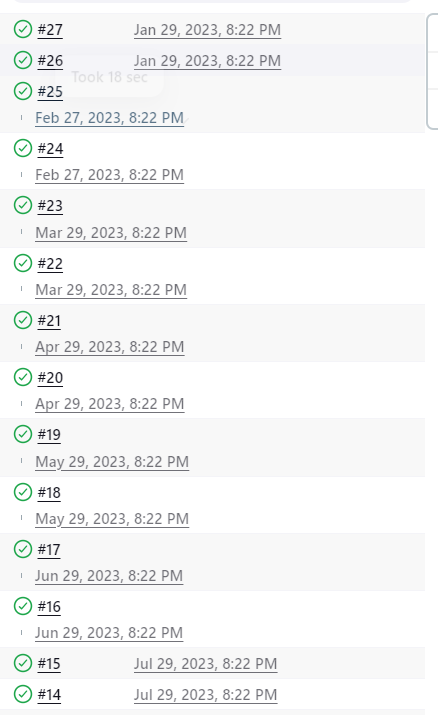
\includegraphics [scale=0.67] {my_folder/images//genetatedBuild}
	\caption{Сгенерированные сборки реального проекта} 
	\label{fig:genetatedBuild}  
\end{figure}

Результаты работы плагина на описанном выше проекте отображены на рисунках 4.7-8. На рисунке 4.7 видно на графике SR, как менялся процент успешности сборок в течении года на столбчатой диаграмме. Также видно на графике BD динамику изменения продолжительности сборок за последний год на линейном графике, в данном случае можно отследить как менялось среднее значение продолжительности. Видно, что время сборки незначительно увеличивалось, т.е. при увеличении кода приложения, в продолжительности сборки также увеличивалось время, за исключением 8 и 11 месяцев. 


 \begin{figure}[ht!] 
	\center
	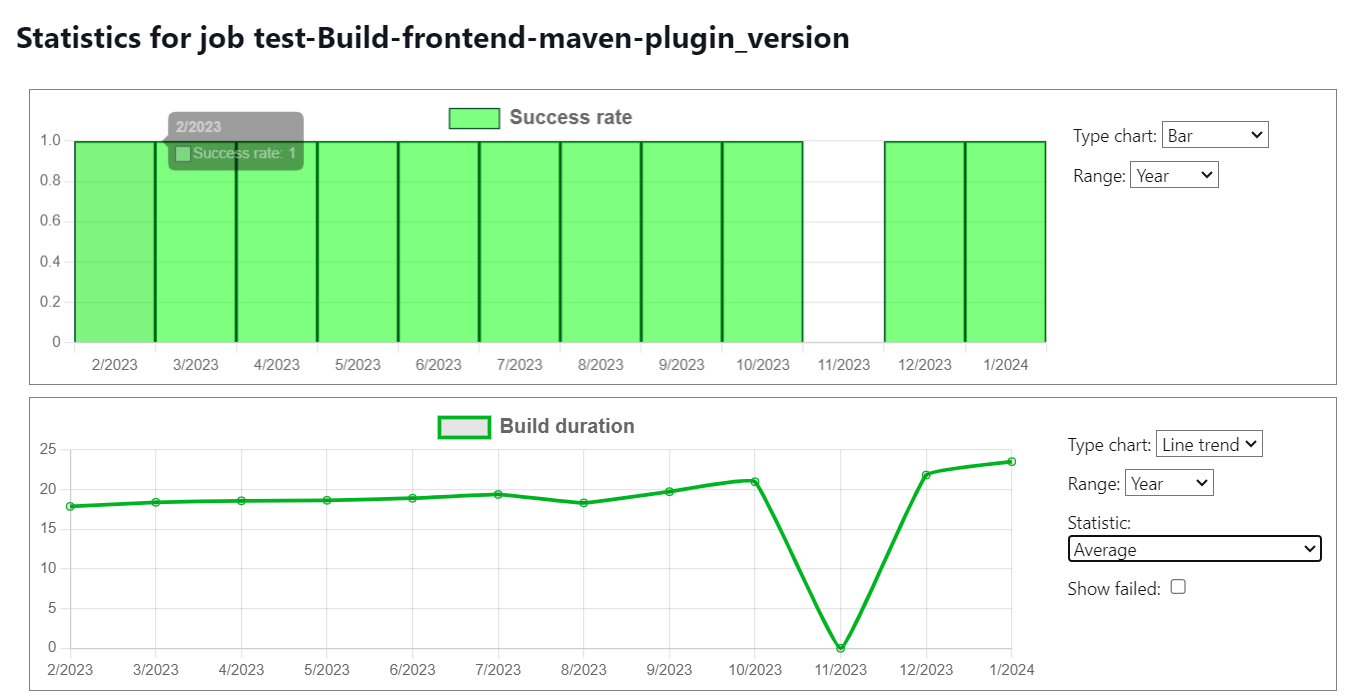
\includegraphics [scale=0.47] {my_folder/images//reares1}
	\caption{Результаты апробации на реальном проекте SR, BD} 
	\label{fig:reares1}  
\end{figure}

В 8 месяце в изменениях кода была повышена версия npm и node, что оптимизировало время выполнения сборки, которое уменьшилось с 19.3 до 18.3 секунд. А версия в 11 месяце, вероятно была не протестировано перед загрузкой в главную ветку, поскольку результат из 3 запусков сборки закончился падением. Что также видно на графике SR, т.е. можно сделать вывод что в коммите был дефект, а не оптимизация, которая ускорила время сборки в несколько раз.

На рисунке 4.8 можно увидеть с помощью радарной диаграммы общий размер, сгенерированных логов-артефактов за последний год. Видно, что с каждым месяцем размер артефактов увеличивался, что также можно объяснить увеличением исходного кода продукта, также наглядна видно разницу между первым и последним месяцем года, а также то что при отображении упавших сборок видно, то что генерировались артефакты, хоть и с небольшим размером.

 \begin{figure}[ht!] 
	\center
	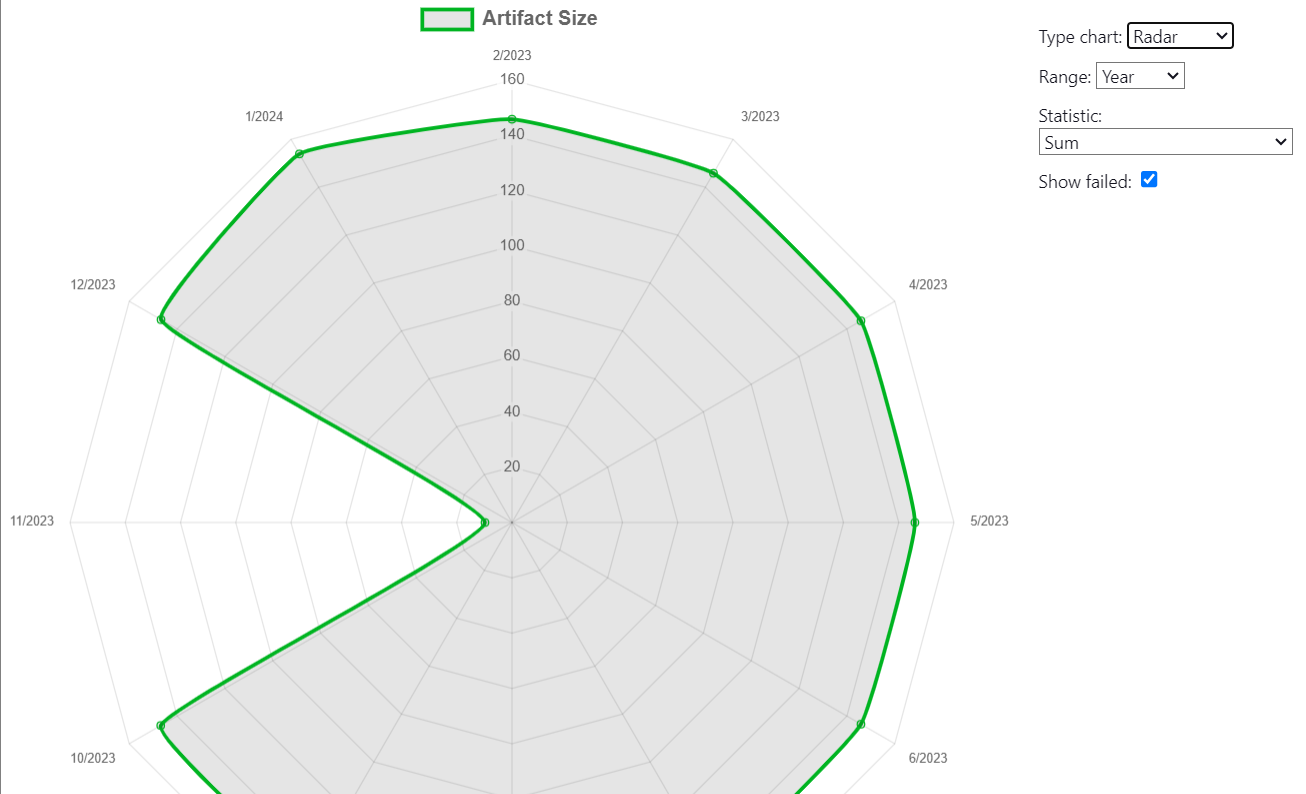
\includegraphics [scale=0.47] {my_folder/images//realres2}
	\caption{Результаты апробации на реальном проекте AS} 
	\label{fig:realres2}  
\end{figure}

По описанным выше результатам визуализации можно прийти к выводу, что плагин полезен тем, что отображает изменение различных метрик запусков сборки с течением времени, т.е. можно увидеть тенденцию изменений в созданных сборках Jenkins в течении цикла разработки за нужный период времени и если метрики в какой момент изменили свои значения, можно определить, что это за момент (или период) и проанализировать как изменения в сборке, тестах или коде могли повлиять на это.

Для удобства пользователей, как видно на рисунках выше, результаты отображаются на разных типах диаграмм, чтобы каждой участник команды мог изучать динамику изменения метрик, так как ему удобно. Также видно, что возле метрик BD, SR, AS можно выбрать статистический показатель, в соответствии с которым будут обработана метрика. Тем самым, можно определить является отклонение случайностью, нестабильностью сборки или это какая-то закономерность.

После анализа разработчики, тестировщики и DevOps-инженеры могут принять решение, насколько критичны данные изменения для процессов CI/CD и если потребуется оптимизировать сборки, тесты или, возможно, какую-то часть кода.

Также по данным диаграммам можно обнаружить и другие проблемы, например, аномалии в процессах сборки или тестирования или окружении, в котором производится сборка или установка компонентов системы.

 \subsection{Оценка результатов работы}
 
 Для того чтобы оценить результаты работы, будет проведено сравнение функционала, который присутствует в аналогичных решениях: плагинах, сравнительный анализ, которых проводился в разделе 1.5 и модуль Statistics, реализованный в средстве CI TeamCity, который и послужил причиной для создания аналогичного модуля в Jenkins.
 
 
 


В разработанном плагине реализовано 7 статистических показателей, которые применяются к метрикам сборок, что является значительным преимуществом в сравнении с аналогичными решениями, поскольку в аналогичных плагинах Jenkins, а также в модуле TeamCity реализован только расчет среднего арифметического значения, и при том не во всех аналогичных плагинах Jenkins.

Также преимуществом разработанного плагина является наличие 3 типов диаграмм для каждой метрики, что больше чем у всех аналогичных решений.

Все результаты сравнения с аналогичными решениями приведены в таблице 4.2.

 \begin{table}
    \centering
    \caption{Количественные результаты работы}
    \begin{tabular}{|p{3cm}|p{3cm}|p{2cm}|p{2cm}|p{2cm}|p{2cm}|}
    \hline
        Критерий & Разработанное решение & TeamCity & Build Monitor Plugin & Global Build Stats Plugin  & Build Time Blame \\ \hline
        Количество визуализируемых метрик & 5 & 5 & 1 & 2 &2 \\ \hline
        Количество статистических показателей & 7 & 1 & 0 & 1 &1\\ \hline
        Количество типов диаграмм & 3 & 2 & 1 & 1 &1\\ \hline


    \end{tabular}
\end{table}

Если сравнивать по количеству визуализируемых метрик, то видно, что все 5 метрик, которые были реализованы в TeamCity, удалось реализовать и в разработанном плагине, аналогичные плагины Jenkins визуализируют определенные из перечисленных в разделе 1.5 метрик, но их количество меньше 5.


 
 
\section{Выводы} \label{ch4:sec3}

После проведения этапа апробации и тестирования плагина визуализации статистики сборок Jenkins можно прийти к выводу, что тестирование проведено в полном объеме и затронуло разные методы, техники тест-дизайна и соответствует методологиям и устоявшимся практикам тестирования программного обеспечения. Апробация протестированного плагина, дала понять, что плагин корректно отрабатывает при разных поданных на вход исходных данных и настройках. Корректно высчитываются и визуализируются статистические показателе обработанных метрик:

\begin{itemize}
	\item среднее арифметическое;
	\item мода;
	\item медиана;
	\item размах;
	\item среднеквадратическое отклонение;
	\item среднеквадратическое отклонение несмещенное;
	\item дисперсия.
\end{itemize}

Визуализация метрик со статистическими показателями была проверена на различных типах диаграмм/графиков:

\begin{itemize}
	\item столбчатая диаграмма;
	\item линейный тренд;
	\item радарная диаграмма.
\end{itemize}

В результате разработки автоматизированных тестов было разработано 22 юнит теста и 8 UI тестов.






%
%

%
%
%\begin{table} [htbp]% Пример оформления таблицы
%	\centering\small
%	\caption{Представление данных для сквозного примера по ВКР \cite{Peskov2004}}%
%	\label{tab:ToyCompare}		
%		\begin{tabular}{|l|l|l|l|l|l|}
%			\hline
%			$G$&$m_1$&$m_2$&$m_3$&$m_4$&$K$\\
%			\hline
%			$g_1$&0&1&1&0&1\\ \hline
%			$g_2$&1&2&0&1&1\\ \hline
%			$g_3$&0&1&0&1&1\\ \hline
%			$g_4$&1&2&1&0&2\\ \hline
%			$g_5$&1&1&0&1&2\\ \hline
%			$g_6$&1&1&1&2&2\\ \hline		
%		\end{tabular}	
%	\normalsize% возвращаем шрифт к нормальному
%\end{table}


% \firef{} от figure reference
% \taref{} от table reference
% \eqref{} от equation reference




